\documentclass[a4paper,11pt]{ijamas}

\renewcommand{\baselinestretch}{1.21}

\usepackage{stfloats}
\usepackage{graphicx}
\usepackage{amssymb}
\usepackage{graphicx}
\usepackage{booktabs}
\newcommand{\ra}[1]{\renewcommand{\arraystretch}{#1}}
\usepackage{amsmath}
\usepackage{algorithm}
\usepackage{algpseudocode}% http://ctan.org/pkg/algorithmicx
\usepackage{epsfig}
\usepackage{tablefootnote}
\usepackage{multirow}
\usepackage{eqnarray}
\usepackage{setspace}
%\usepackage{natbib}
\usepackage{url}
\usepackage{booktabs}

%\usepackage{graphicx}
%\usepackage{caption}
%\usepackage{subfig}
\usepackage{booktabs}
\usepackage{subcaption}

\usepackage{blindtext}

\usepackage{threeparttable, tablefootnote}
\newcommand{\normal}[1]{\multicolumn{1}{l}{#1}}
\newcommand{\head}[1]{\textnormal{\textbf{#1}}}
\addtolength{\parskip}{-1mm}
%
% \usepackage{mathptmx}      % use Times fonts if available on your TeX system
%
% insert here the call for the packages your document requires
%\usepackage{latexsym}
% etc.
%
% please place your own definitions here and don't use \def but
% \newcommand{}{}
%
% Insert the name of "your journal" with
% \journalname{myjournal}
%
\usepackage{caption}

\captionsetup[algorithm]{font=footnotesize}

%=====


\begin{document}

%%%%%%%%%%%%%%%%%%%%%%%%%%%%%%%%%%%%%%%%%%%%%%%%%%%%%%

\title{A Preprocessing Scheme for Fluorescence Microscopy Image Segmentation}

\author{\textbf{Ryan Naidoo$^1$ and Jules-Raymond Tapamo$^1$}}

\date{$^1$School of Engineering\\
University of KwaZulu-Natal\\
Durban, 4041, South Africa\\
rai5395@gmail.com,tapamoj@ukzn.ac.za}

\maketitle

%%%%%%%%%%%%%%%%%%%%%%%%%%%%%%%%%%%%%%%%%%%%%%%%%%%%%%



%%%%%%%%%%%%%%%%%%%%%%%%%%%%%%%%%%%%%%%%%%%%%%%%%%%%%%%

\begin{abstract}

\noindent \emph{Significant technological advancements in image acquisition and enhancement techniques together with significant advancements and results in fluorescence microscopy have lead to an overload of image data, which, on any level of tractability in time and quality, is too much to be analysed manually. There is a natural demand for highly accurate automated analysis. In spite of the significant advancements, there are still problems that present themselves in a way that makes high level analysis difficult. Typically, image analysis is preceded by segmenting the regions of interest. In our case we are concerned with cells (and possibly intracellular components), bacteria, etc. This necessitates a greater degree on the quality of segmentation algorithms. This paper proposes a preprocessing scheme to draw out and enhance edge and intra-region properties to allow more accurate segmentation. This scheme is tailored towards fluorescence images but can be applied to other domains. The final segmentation results show a general boost in classification accuracy as well as a smoother fitting of the contour around the cells.}
\medskip

\noindent\textbf{Keywords:} Coherence enhancing diffusion, fluorescence microscopy, segmentation, total variation denoising.

\medskip

\noindent\textbf{Computing Classification System (CCS):} I.4.3, I.4.6, J.3.

\end{abstract}





\section{Introduction}
\label{sec:intro}
Fluorescence microscopy has become an indispensable tool \cite{pmatula:2012} in myriad of scientific disciplines such as chemistry, biology, neurobiology and medicine to name a few. It gives scientists visual access to physiological processes and other cellular and sub-cellular activities.
Fluorescence microscopy coupled with the tremendous technological advancement of image acquisition has lead to an explosion of raw image data such that the sheer volume of images acquired presents too much of a burden on manual analysis \cite{pmatula:2012}.
Consequently, there is a need for highly accurate automated analysis.
In such image analysis, image segmentation has established itself as a key process in identifying and extracting objects of interest which can thereafter be used in higher level image analysis.
The ever increasing demand on image segmentation is to extract the objects of interest with greater accuracy in a shorter time.

There are many factors that degrade the quality of fluorescence images and these can result in sub-optimal segmentations.
%affect the accuracy of the segmentation.
These factors have been studied independently to a great deal and have been successfully applied to real-world data.
Some of these problems are poor contrast, photo-bleaching, a not black enough blackground, non-fluorescence of samples, improper excitation, etc.

Literature is rich with techniques that are able to, a high degree, negate the effect of these factors \cite{lysaker:2004,wang:2008,zhou:2013}. There is, however, a lack of definition of a scheme prior to segmentation that prepares an image such that accurate segmentation can be achieved.

The task of defining a set of criteria an image has to meet for reliable segmentation results is not a trivial one. However, there are some basic notions that an image can be tuned towards which would present a better image for the purpose of segmentation.
%obtained,
Image enhancement on the original image can be done to facilitate higher level analysis e.g. contrast enhancement.
%segmentation qualities. The criteria of this scheme is
This paper aims to design a hybrid algorithm that builds on highly successful algorithms to produce better results. The process emphasises
\begin{enumerate}
\item Noise reduction
\item Object data enhancement
\item Edge completion and enhancement
\item Reduction of intra-region variance
\end{enumerate}

The remainder of this paper is organised as follows: In \autoref{sec:background} we discuss the background and related work. The proposed scheme is presented in \autoref{sec:proposed}. We present the experimental results in \autoref{sec:results} and conclude in \autoref{sec:conclusion}.


\section{Background}
\label{sec:background}
One of the most common forms of image corruption is noise. A large number of denoising algorithms assume the image to be corrupted by a stationary additive zero mean Gaussian noise (AWGN) \cite{rodriguez:2008,le:2005,luiser:2011}. In this scenario the observed image $y$, is modelled as signal-independent as follows:
\begin{equation}
 y = x + \epsilon
\end{equation}
where $\epsilon$ is the Gaussian random variable that captures that statistical noise of the system.
The Gaussian function is defined as:
\begin{equation}
G(x) = \frac{1}{\sigma\sqrt{2\pi}} e^{-\frac{(x-\mu)^2}{2\sigma^2}}
\end{equation}
Where $\sigma$ is the standard deviation and $\mu$ is the mean.
However, medical images are often corrupted by other types of non-Gaussian noise.

The dominant forms of noise present in medical imaging, such as positron emission tomography (PET), single photon emission computed tomography (SPECT), and confocal fluorescent microscopy \cite{rodriguez:2008}, is photon noise and dark noise \cite{luiser:2011,le:2005}. This is due to the acquisition process and the physical mechanisms involved \cite{luiser:2011,le:2005}.

Photon noise, also known as photon-shot noise, is the signal dependant statistical variations of a signal composed from counting the number of quanta incident on a film or CCD. This natural phenomenon cannot be reduced by camera design.
Dark current refers to the rate at which extraneous electrons are excited, due to thermal energy, into a signal. This signal also carries statistical fluctuation known as dark noise.
Both photon noise and dark noise is Poisson distributed.
Denoising has been a topic of interest for many years and the evidence of its popularity is the abundance of techniques, models and algorithms that have been developed; more details can be found in \cite{luiser:2011,luiser:2009,raj:2012,raj2:2012,shinde:2012,raj3:2012,garg:2012}.

% need to quote some guys here
Another significant problem in the images obtained through fluorescence microscopy is low contrast and limited dynamic range \cite{olympusmicro1:2012}. Generally, it is easier to discriminate object from one another if there is very little similarity, with regards to the feature under critique, between them. Thus, low contrast images is a problem that needs to be looked at thoroughly. Just like denoising, the topic of contrast enhancement has also been well researched and the literature on the subject is abundant \cite{khellaf:1991,stark:2000,starck:2003,celik:2012,mukherjee:2009}.

% need to quote some guys here
An important factor to take into account in segmentation is edge enhancement and edge completion. The edges of the objects of interest in fluorescent microscopy tend to suffer from non-uniform lighting and is often disjointed \cite{olympusmicro2:2012}. In this regard, many state-of-the-art segmentation algorithms will produce a non-ideal segmentation contour due to the fact that the input image has missing edge information or the edge information is not "strong" enough to be considered a valid edge. Hence, this problem needs to be considered before the segmentation technique is applied.

\section{Proposed Scheme}
\label{sec:proposed}
In this section we present a novel scheme which enhances the image such that it has better segmentation qualities. It is tailored towards images obtained from fluorescence microscopy. The proposed scheme is shown in Figure \ref{fig:proposed_framework}. The effect of each stage in the framework is shown using Figure \ref{fig:test_orig} as the test image. The first two steps deal primarily with noise reduction, steps three and four deal primarily with bringing out the object and the final step deals with edge enhancement, edge completion and reducing intra-region variance. The ensuing subsections provide a deeper look into steps involved.

\begin{figure}[!t]
\centering
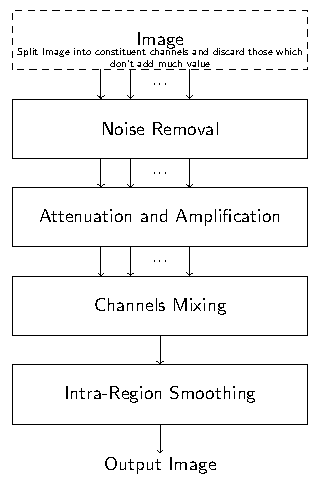
\includegraphics[width=0.80\columnwidth]{./figs/5.pdf}
\caption{Proposed Preprocessing Framework.}
\label{fig:proposed_framework}
\end{figure}



\subsection{Discard Noise-only Channels}
\label{sec:proposed_remove_channels}
Many segmentation algorithms are designed to work on gray scale images. If we have a colour image it is first converted to gray scale. Through the advancements in optical engineering it is now possible for fluorescence images to be obtained in colour, however not all channels add object data to the image. They in fact degrade the image due to the noise in that channel.
A direct conversion of the colour image to a gray scale image yields poor results as seen in Figure \ref{fig:test_gray}. In Figure \ref{fig:test_orig}, there is clearly no blue-channel data in the image, as a result when the image is converted to gray scale, as shown in Figure \ref{fig:test_gray}, the red-channel data is significantly suppressed due to the averaging of the channels that occurs when the conversion to gray scale takes place. Most of the times a redundant channel will just be composed of noise and eliminating this channel will provide a huge improvement to the image. In this case, the redundant blue-channel can be discarded entirely which yields Fig. \ref{fig:test_chanmixgray}.




\subsection{Noise Removal}
\label{sec:proposed_noise_removal}
In \autoref{sec:background} we mentioned that the primary forms of noise in fluorescent images is Poisson noise. It is important that when applying the denoising filters the boundary information, i.e. edges, is not lost or degraded. A visual analysis can show to which degree the edge information has been affected.
We used the Total-Variation Anisotropic denoising (Bregman Split) since it removes noise and preserves edges most effectively as shown in \cite{rodriguez:2008}. Although it was developed to remove Gaussian noise, it performs better at removing Poisson noise than many state-of-the-art Poisson denoising filters \cite{rodriguez:2008,michelli:2011} such as wavelets \cite{timmermann:1999}, platelets\cite{willett:2004}, minimum description length \cite{nowak:1999}.

The Poisson distribution, which has equal mean and standard deviation i.e. $\mu = \sigma$, is defined by
\begin{equation}
	P(n,\mu) = \frac{e^{-\mu}\mu^{n}}{n!}
	\label{eq:poissondist}
\end{equation}

Let $y = \lbrace y_i:i=1, \cdots, N \rbrace$ and $x = \lbrace x_i:i=1, \cdots, N \rbrace$ be the observed and the true image, respectively. The sample $y_i$ is a Poisson contaminated form of $x_i$. We desire to recover the signal $x$ from the observed signal $y$. From Bayes' Law we get
\begin{equation}
	P(x \vert y) = \frac{P(y \vert x)P(x)}{P(y)}
	\label{eq:bayeslaw}
\end{equation}
Therefore, we wish to find the maximum of $P(y \vert x)P(x)$. If all samples are affected by Poisson noise we have
\begin{equation}
	P(y \vert x) = P(y,x) = \frac{e^{-x_i}x_i^{y_i}}{y_i!}
	\label{eq:poissonafect}
\end{equation}
Thus the likelihood of observing $y$ given the true image $x$ is given by
\begin{equation}
	P(y \vert x) = \prod_{i=1}^{N} \frac{e^{-x_i}x_i^{y_i}}{y_i!}
	\label{eq:poissonlikelihood}
\end{equation}


In anisotropic TV denoising we wish to recover the original image given the noisy image by minimising the constrained problem

\begin{equation}
\underset{u} {\mathrm{min}} \left| \left| \frac{du}{dx} \right| \right|_1 + \left| \left| \frac{du}{dy} \right| \right|_1 + \frac{\mu}{2} \left| \left| u-f \right| \right|^2_2
\label{equ:anisotropic_tv_constrained}
\end{equation}
where $\mu > 0$ is the regularisation parameter which affects the balance between noise removal and signal preservation \cite{getreuer:2012}, $u$ is the true image and $f$ is the noisy image. We actually solve the unconstrained problem
\begin{multline}
\underset{u, dx, dy} {\mathrm{min}} \left| \left|dx_1 \right| \right|_1 + \left| \left| dy_1 \right| \right|_1 + \frac{\mu}{2} \left| \left| u-f \right| \right|^2_2 +
 \frac{\lambda}{2} \left| \left| dx-u_x \right| \right|^2_2 + \frac{\lambda}{2} \left| \left| dy-u_y \right| \right|^2_2
\label{equ:anisotropic_tv_unconstrained}
\end{multline}
This can be solved using the Bregman Split algorithm \cite{wei:2010}.
The algorithm is run iteratively until the error, $e = \frac{\vert u'-u \vert}{\vert u \vert}$ where $u'$ is the image obtained after denoising the input image $u$, is less than a user-defined tolerance factor, $\epsilon$. We used  $\mu=20$, $\lambda=1$ and $\epsilon=1 \times 10^{-3}$, the original and the denoised channels are shown in Figures \ref{fig:gchannel_1_orig}, \ref{fig:rchannel_1_orig}, \ref{fig:gchannel_1_denoised} and \ref{fig:rchannel_1_denoised}

\begin{figure}[!h]
\centering
\begin{subfigure}{.48\textwidth}
  \centering
  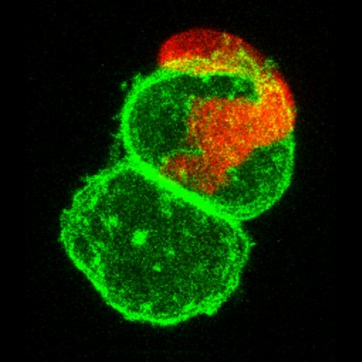
\includegraphics[width=0.80\columnwidth]{./figs/_2colr.jpg}
 \caption{Original \cite{cil:11996}}
  \label{fig:test_orig}
\end{subfigure}%


\begin{subfigure}{.48\textwidth}
  \centering
  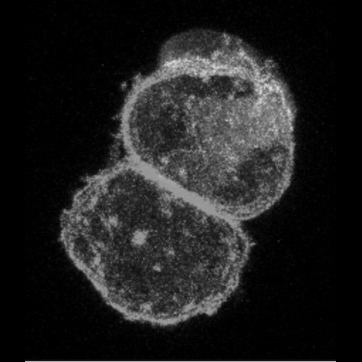
\includegraphics[width=0.80\columnwidth]{./figs/_2gray.jpg}
 \caption{RGB channels gray scale conversion}
  \label{fig:test_gray}
\end{subfigure}%
\begin{subfigure}{.48\textwidth}
  \centering
  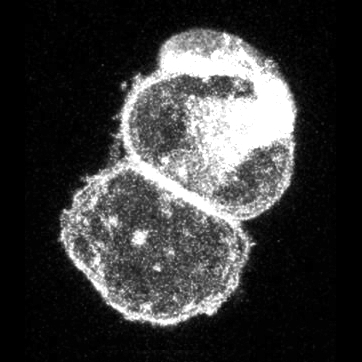
\includegraphics[width=0.80\columnwidth]{./figs/_2chanmixgray.jpg}
 \caption{Red-Green channels gray scale conversion}
  \label{fig:test_chanmixgray}
\end{subfigure}%
\caption{Test image original, gray scale, gray scale without blue-channel}
\end{figure}

\subsection{Data Attenuation and Amplification}
\label{sec:proposed_remapping}
For highly successful segmentation, it is preferred that there is enough difference between the object and the background, in some feature on which a particular segmentation algorithm is designed. In gray level images, this feature is typically the gray level intensity.
With regard to segmentation, an "ideal" image is one that can be mapped to a feature space where the feature that determines the object and the background do not overlap. However, in medical images this is never the case since such a feature space is not known or doesn't exist. In this regard there is always some overlap in the subsets that represents the background and the object.
This overlap presents the most uncertainty in classifying a pixel.

Contrast enhancement is a common tool used in medical image processing, as shown in \cite{kim:2003} and \cite{subr:2005}, and it would be easy to see why such a technique would elude to be thought of as belonging to a pre-processing scheme since the aim of contrast enhancement is to bring out hidden details in an images that are otherwise lost due to a low dynamic range, improper lighting, etc.
Contrast enhancement may make it easier to see an image but it does not directly move the image to that of an "ideal" image for segmentation.

In this section we present a novel data remapping function that works on the gray level intensity of an image.
In this regard, it is trivial that if there is a greater disparity in gray values between the object and the background then a segmentation algorithm would yield less false positives and negatives.
In this regard the pixel value that has the most uncertainty would generally split the dataset into two subsets. These are the background dataset and the object dataset.



\begin{figure}[!h]
\begin{subfigure}{.48\textwidth}
  \centering
  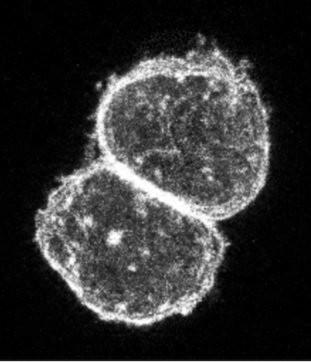
\includegraphics[width=0.80\columnwidth]{./figs/2aG.jpg}
 \caption{Original green channel}
  \label{fig:gchannel_1_orig}
\end{subfigure}%
\begin{subfigure}{.48\textwidth}
  \centering
  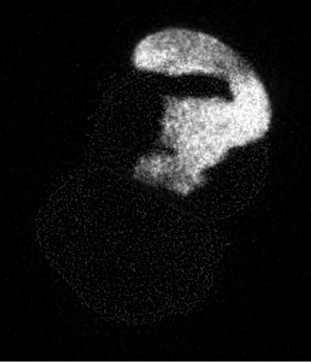
\includegraphics[width=0.80\columnwidth]{./figs/2aR.jpg}
 \caption{Original red channel}
  \label{fig:rchannel_1_orig}
\end{subfigure}%

\begin{subfigure}{.48\textwidth}
  \centering
  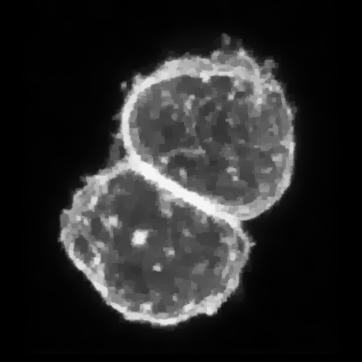
\includegraphics[width=0.80\columnwidth]{./figs/2bG.jpg}
 \caption{Denoised green channel}
  \label{fig:gchannel_1_denoised}
\end{subfigure}%
\begin{subfigure}{.48\textwidth}
  \centering
  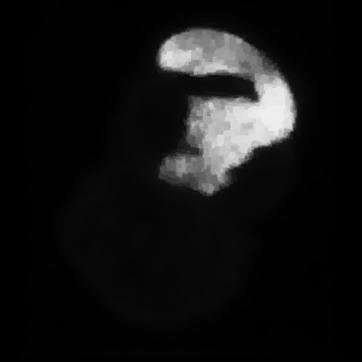
\includegraphics[width=0.80\columnwidth]{./figs/2bR.jpg}
 \caption{Original red channel}
  \label{fig:rchannel_1_denoised}
\end{subfigure}%
\caption{Original and denoised channels}
\label{Flo:cell_positions_and_shape}
\end{figure}

\subsubsection{Function Criteria}
\label{sec:functioncriteria}

We define the criteria needed to remap the image such that object data is amplified and background data is attenuated. We then design a function based on this criteria as follows: \\ \\
\underline{Criteria for the Design of the Mapping Function}\\
The remap function is denoted as $\widetilde{x_i} = R(x_i)$, where $\widetilde{x_i}$ is the new value which remaps the input pixel, $x_i$, using the function $R$. The range on which $R$ works is $[0,L]$, where $0$ and $L$ represent the lowest and highest values a pixel can take respectively. For 8-bit gray scale images the highest value is usually $L=255$. The value that represents the greatest classification uncertainty is denoted as $N$.
\begin{enumerate}
\item{}
\textit{$R$ must be non-decreasing in the interval $[0, L]$}\\
This is a trivial criterion arising from the fact that it is not possible for a pixel of a lower gray level intensity to have a higher probability of belonging to the object than for a pixel of a higher gray level intensity. However, due to discretisation, more than one pixel may be mapped to the same gray level intensity.

\item
\textit{$\widetilde{x_i} = R(x_i=N) = N$}\\
Since this value presents the most uncertainty, there is no bias as to whether it tends more to the background or the object. It is best left unaltered.

\item
\textit{Attenuation: $\widetilde{x_i} < x_i, \, \forall x_i<N$}\\
$R$ must remap gray-level intensities below the value of greatest uncertainty, $N$, according to $0 \leq \widetilde{x_i} \leq x_i$.

\item
\textit{Amplification: $\widetilde{x_i} > x_i, \, \forall x_i>N$}\\
$R$ must remap gray-level intensities above the point of greatest uncertainty, $N$, according to $x_i \leq \widetilde{x_i} \leq L$.

\item
\textit{$R'$ must be non-decreasing in the interval $[0,N]$}\\
Given two pixels, $p_1$ and $p_2$, with values $x_1$ and $x_2$ respectively where $x_1<x_2$. It is more probable for $p_2$ to belong to the object since it has a higher value. Conversely, pixels with gray levels intensities closer $0$ do not need to be attenuated as much.

\item
\textit{$R'$ must be non-increasing in the interval $[N,L]$}\\
As the pixels values approach $L$, less amplification is needed since the pixels are already more likely to be classified as belonging to the object.

\end{enumerate}
\subsubsection{Function Design}
Many functions can be designed given the criteria in Section \ref{sec:functioncriteria}. It is important however, to maintain easy and intuitive tuning of the mapping function. This is easily attained by making the mapping function piece-wise quadratic bezier curve.
\\
The remapping function will be composed of two functions which are $R_{att}$, for the attenuation section, and $R_{amp}$, for the amplification section as shown in Figure \ref{fig:mapping_plot}



There are three anchor points which the function passes through. These are $p_0(0,0)$, $p_2(N, N)$ and $p_4(L,L)$. If the curve lies on the line that passes through the anchor points then there is no change between the output image and the input image. Additional control points are needed to bend the curve.
There are only certain shapes of the curve which are desired. This presents constraints on the position of the control points. Relative to the totally relaxed curve, $y=x, \, x \in [0,L]$, the amplification curve would be above the relaxed line, $p_{3y} > p_{3x}$, and similarly the attenuation curve would be below the line, $p_{1y} < p_{1x}$. Also, given that the function is to be a one-to-one function, the control point for the attenuation function $p_{1x}<N$; similarly the control point for the amplification function $p_{3x}>N$.


\begin{figure}[!h]
\centering
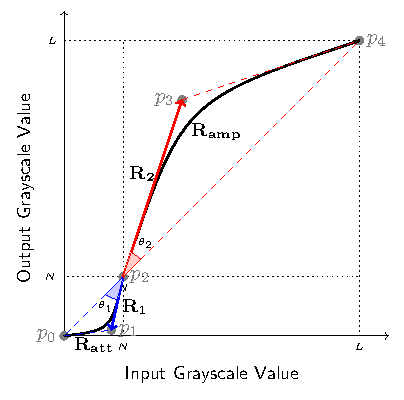
\includegraphics[width=0.80\columnwidth]{figs/remapfcn.pdf}
\caption{Plot of remapping function.}
\label{fig:mapping_plot}
\end{figure}

The controls points in the Cartesian representation don't say much about the amount of tension in the curve. A more useful representation is to represent the control point implicitly as an angular deviation of the relaxed curve and a magnitude, $p_c(R_c, \theta_c)$. Where $\theta_c \in [0, \frac{\pi}{4}]$ and $R_c \in \mathbb{R}^+$. This deviation is the measure of the relaxed curve which is counter-clockwise for the amplification function and clockwise for the attenuation function. The deviation, $\theta_c$ of the relaxed curve is further implicitly represented as a range $\kappa_c \in [0,1]$ where $\kappa_c=0$ implies $\theta_c = 0$ would mean no deviation, and $\kappa_c = 1$ implies $\theta_c = \frac{\pi}{4}$ would mean maximum deviation.
The advantage in defining the function is that it gives a geometric intuition to the rate of change of probability along the curve. As the curve approaches the end of the domain, less attenuation/amplification can occur due to the fact that that pixel already lies in a correct subset.

\begin{figure}[!t]
\begin{subfigure}{.48\textwidth}
  \centering
  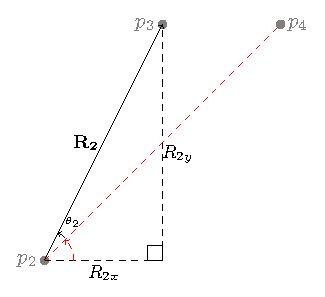
\includegraphics[width=0.80\columnwidth]{figs/3.pdf}
 \caption{Amplification function controls points}
  \label{fig:ampcontrolpoints}
\end{subfigure}%
\begin{subfigure}{.48\textwidth}
  \centering
  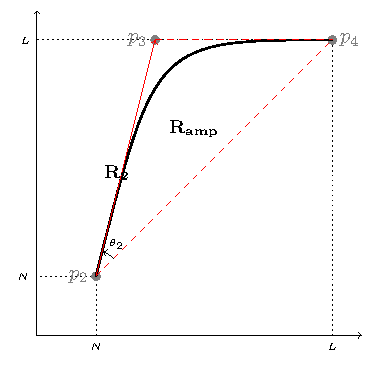
\includegraphics[width=0.80\columnwidth]{figs/4.pdf}
 \caption{Amplification function curve}
  \label{fig:ampcurve}
\end{subfigure}%
\caption{Amplification function control points and curve.}
\label{fig:ampcalculation}
\end{figure}

The position of the attenuation control point is calculated as
\begin{equation*}
{p_1} = \left(
		p_{2x} - R_1\cos[\frac{\pi}{4}(1+\kappa_1)],
		p_{2y} - R_1\sin[\frac{\pi}{4}(1+\kappa_1)]
		\right)
\end{equation*}
%\begin{multline*}
%{p_1} = \left(
%		p_{2x} - R_1\cos[\frac{\pi}{4}(1+\kappa_1)],
%		p_{2y} - R_1\sin[\frac{\pi}{4}(1+\kappa_1)]
%		\right)
%\end{multline*}
%Similarly, the control point for the amplification function is given by
Similarly, the position of the amplification control point, as shown in Figure \ref{fig:ampcalculation}, can be calculated as
\begin{equation*}
{p_3} = \left(
	p_{2x} + R_2\cos[\frac{\pi}{4}(1+\kappa_2)],
	p_{2y} + R_2\sin[\frac{\pi}{4}(1+\kappa_2)]
\right)
\end{equation*}

The piecewise functions that define the curve are given by	
\begin{eqnarray}
	R_{att}(t) = \sum_{i=0}^2 p_i J_i^n \\
	R_{amp}(t) = \sum_{i=2}^4 p_i J_i^n
\end{eqnarray}
Where $J_i^n$ is the Bernstein basis function, defined as
\begin{equation}
	J_i^n = \begin{pmatrix}
				n \\
				i
			\end{pmatrix}	
			t^i(1-t)^{n-i}, \,\, t \in [0,1]
	\label{eq:bernsteinbasis}
\end{equation}
For each input gray level intensity $x \in [0, L]$ we require corresponding output gray level intensity $y \in [0, L]$.
The curve is expressed as a parametrisation with respect to $t$ for each of its $x$ and $y$ parameters.
For a curve defined by three control points $q_0$, $q_1$ and $q_2$ where $q_0 < q_1 < q_2$, the equation for the curve determine by these points is the quadratic bezier given by
\begin{equation}
	R = \sum_{i=0}^2 q_i J_i^n
\end{equation}

For a quadratic bezier curve, this simplifies to
\begin{align*}
	R &= q_0(1-t)^2 + 2q_1(1-t)t + q_2t^2 \\
	0 &= (q_0-2q_1+q_2)t^2 + (-2q_0+2q_1)t + (q_0-R)
\end{align*}
Therefore for the parametric function $R_x$, we require the set of values of $t$ for which $R_x \in [q_{0x},q_{2x}]$. The value of $t$ for a given $R_x$ is determined by the solution to the quadratic equation.\\
Let $a=q_{0x}-2q_{1x}+q_{2x}$, $b=-2q_{0x}+2q_{1x}$, and $c=q_{0x}-R_x$.\\
It is seen that $b>0$, since $q_{1x} > q_{0x}$, and $c \leq 0$, since $R_x \geq q_{0x}$.\\
Rewrite $a$ as $a=(q_{0x}-q_{1x}) + (q_{2x}-q_{1x})$.
For the case of $a$, there are two cases.\\
\begin{enumerate}
\item
For $q_{1x} \in [q_{0x}, \frac{q_{2x}-q_{0x}}{2}]$, $a>0$.\\
In this case $-4ac>0$ hence $\sqrt{b^2-4ac}>b$.\\
$\therefore$ the only value of $t$ which is positive and must be the solution is given by

\begin{equation}\label{qt1}
 t =  \frac{(q_{1x}-q_{0x})+\sqrt{R_x(q_{0x}-2q_{1x}+q_{2x})+(q_{1x}^2-q_{0x}q_{2x}})}
		{q_{0x}-2q_{1x}+q_{2x}}
\end{equation}
%\begin{multline}
%t =  \frac{(q_{1x}-q_{0x})+\sqrt{R_x(q_{0x}-2q_{1x}+q_{2x})+(q_{1x}^2-q_{0x}q_{2x}})}
%		{q_{0x}-2q_{1x}+q_{2x}}
%\end{multline}



\item
For $q_{1x}>\frac{q_{2x}-q_{0x}}{2}$, $a<0$.\\
It is known that a real solution exists. This means that
\begin{align*}
	b^2 -4ac &\geq 0 \\
	b^2 &\geq 4ac \\
	\implies \sqrt{b^2-4ac} &< b
\end{align*}
$\therefore$ the only value of $t$ which is positive and must be the solution is given by

%\begin{multline}
%t =  \frac{(q_{1x}-q_{0x})+\sqrt{R_x(q_{0x}-2q_{1x}+q_{2x})+(q_{1x}^2-q_{0x}q_{2x}})}
%		{q_{0x}-2q_{1x}+q_{2x}}
%\end{multline}
\begin{equation}\label{qt2}
 t =  \frac{(q_{1x}-q_{0x})+\sqrt{R_x(q_{0x}-2q_{1x}+q_{2x})+(q_{1x}^2-q_{0x}q_{2x}})}
		{q_{0x}-2q_{1x}+q_{2x}}
\end{equation}


\end{enumerate}
In both cases the solution to $t$ can be calculated using the same formula.
It is possible for the remapping function to exceed the range, in this case any value that maps to a value higher than the maximum value will be assigned the maximum value i.e. $\widetilde{x_i} = min(R(x_i),L), \,  x_i \in (N,L]$; similarly any value that maps to a value lower than the minimum value will be assigned the minimum value i.e. $\widetilde{x_i} = max(R(x_i),0), \, x_i \in [0,N)$.

\subsubsection{Function Properties and Constraints}
This function presents several properties within the constraints defined a follows:
\begin{enumerate}
\item
The curves obey the convex hull property. The sub-functions will always be contained within the control polygon determined by the control points \cite{jvince:2006,dmarsh:2005}.

\item
No attenuation when $\kappa_1=0$ and no amplification when $\kappa_2=0$. This is when the curve is completely relaxed.

\item
The curve is continuous in the range $[0,L]$.

\item
The remapping function, $R$, is weakly monotonically increasing.

\item
The first derivative of the attenuation function, $R'_{att}$, is monotonically increasing in $x \in [0, N]$.

\item
The first derivative of the amplification function, $R'_{amp}$, is monotonically decreasing in $x \in [N, L]$.

\item
The ends of the curve are coincident with the first and last control points of the control polygon.

\item
The direction of the tangent vectors from the end points of the curve are the same as the direction of the vector anchored at the control point and along the line that joins the end point and the centre control point of the control polygon.
\end{enumerate}



\subsection{Channel Mixing}
\label{sec:proposed_channelmixing}
At this point all the channels are considered to have very little noise and can be recombined into a single monochrome image. Generally, each channel contributes equally to the mixed-down image.
An equi-weighted mixing system doesn't always produce the best image. A consequence, of equi-weighted mixing is that some channels might become very suppressed and may be disregarded by the segmentation algorithm. Hence, it is necessary to assign weights which are channel dependant. We used $w_R=0.5$, $w_G=0.5$, and $w_B=0.0$ to produce Figure \ref{fig:mixingchannels}, where $w_X$ is the contribution of channel X to the mixed-down image. These weightings must sum to one, $\sum_{i \in C} w_i = 1$, where $C$ is the set of channels to be mixed-down. The mixed-down image is thus calculated as $y = \sum_{i \in C}w_iC_i$, where $C_i$ is channel $i$. Channels with very low gray level values are generally given a greater weight.


\begin{figure}[!h]
\centering
\begin{subfigure}{.48\textwidth}
  \centering
  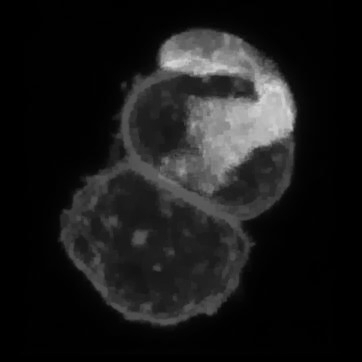
\includegraphics[width=0.80\columnwidth]{./figs/2bRG.jpg}
 \caption{Equi-weighted mixing}
  \label{fig:equimix}
\end{subfigure}%
\begin{subfigure}{.48\textwidth}
  \centering
  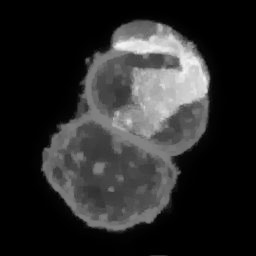
\includegraphics[width=0.80\columnwidth]{./figs/2remapped.jpg}
 \caption{Non-equal channel mixing}
  \label{fig:ampcurve}
\end{subfigure}%
\caption{Equi-weighted mixing versus Non-equi-weighted mixing.}
\label{fig:mixingchannels}
\end{figure}


\subsection{Intra-Region Smoothing}
\label{sec:proposed_ced}

One of the criteria which is used in identifying an image is that objects tend to have little intra-region variance. In medical imaging it is not uncommon to have objects that lack a definite coherent boundary with large luminance variation. This is caused by number of reasons which vary from improper excitation, non-fluorescence of particles to the ubiquitous measurement errors during acquisition. In some cases it is easy to visualise the completed edge of the object by joining the disconnected edge components where the extension is along the direction of the edge.
We used a coherence enhancing diffusion filter presented in \cite{jweickert:1999}, \cite{jweickert:2002} and \cite{jweickert:1998} which very successfully reduces intra-region variance and joins closely-disconnected edges.

The diffusion works by evolving the image, $u$, over a time using $n$ discrete time steps, $t$, called the diffusion time. The evolution equation is defined as:
\begin{equation}
\frac{\partial u}{\partial t} = \nabla \cdot (D\nabla u)
\end{equation}
where $D = \begin{pmatrix}
a & b \\
b & c
\end{pmatrix}$ is the diffusion tensor which can be adapted to the local image structure measure known as the structure tensor. The structure tensor is given by:
\begin{equation}
J_{\rho}(\nabla u_{\sigma}) = G_{\rho} \ast (\nabla u_{\sigma} \nabla u_{\sigma}^T)
\end{equation}
Where $G_{\rho}$ is the Gaussian kernel with standard deviation $\rho$, and $u_{\sigma} := G_{\sigma} \ast u$ where $G_{\sigma}$ is the Gaussian kernel with standard deviation $\sigma$.
The eigenvalues of $J_{\rho}=\begin{pmatrix}
J_{11} & J_{12} \\
J_{12} & J_{22}
\end{pmatrix}$ are
\begin{eqnarray}
\mu_{1} = \frac{1}{2}\left( J_{11} + J_{12} + \sqrt{(J_{11}-J_{22})^2+4J_{12}^2} \right) \\
\mu_{2} = \frac{1}{2}\left( J_{11} + J_{12} - \sqrt{(J_{11}-J_{22})^2+4J_{12}^2} \right)
\end{eqnarray}
Where the normalised first eigenvector satisfies
\begin{equation}
\begin{pmatrix}
cos \alpha \\
sin \alpha
\end{pmatrix} \parallel
\begin{pmatrix}
2J_{12} \\
J_{22}-J_{11}+\sqrt{(J_{11}-J_{22})^2 + 4J_{12}^2}
\end{pmatrix}
\end{equation}
The diffusion tensor's, $D$, eigenvectors are obtained from the structure tensor eigenvectors using:
\begin{eqnarray}
\lambda_1 &=& c_1 \\
\lambda_2 &=& \left\lbrace \begin{matrix}
c_1 & \text{if } \mu_1=\mu_2 \\
c_1+(1-c_1)e^{\frac{c_2}{(\mu_1-\mu_2)^2}}& \text{otherwise}
\end{matrix}
\right.
\end{eqnarray}
where $c_1 \in (0,1)$, $c_2>0$. The elements of $D$ are then calculated as:
\begin{eqnarray}
a = \lambda_1 cos^2 \alpha + \lambda_2 sin^2 \alpha \\
b = (\lambda_1 - \lambda_2)sin \alpha cos \alpha \\
c = \lambda_1 sin^2 \alpha + \lambda_2 cos^2 \alpha
\end{eqnarray}
Further details on the coherence enhancing diffusion filter with optimised rotational invariance is found in \cite{jweickert:2002}.

In \cite{mmaska:2013} and \cite{dkroon:2009} this filter was used primarily for noise removal while preserving edge detail, here we use it for its edge completion and smoothing ability.
The comparison between the original image and the final image is shown in Figure  \ref{Org_dif}, the diffused image appears very distorted however the data necessary for the object extraction is present with less intra-region variance and better edge coherence. These added qualities are vital to yield optimal segmentations.


\begin{figure}[!h]
\centering
\begin{subfigure}{.48\textwidth}
  \centering
  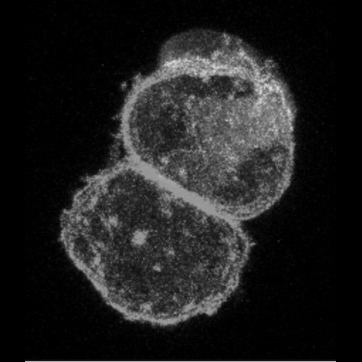
\includegraphics[width=0.80\columnwidth]{./figs/_2gray.jpg}
 \caption{Original gray scale}
  \label{fig:test_original}
\end{subfigure}%
\begin{subfigure}{.48\textwidth}
  \centering
  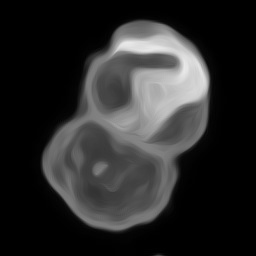
\includegraphics[width=0.80\columnwidth]{./figs/2diffused.jpg}
 \caption{Output image}
  \label{fig:diffused_1}
\end{subfigure}%
\caption{Original image compared to final image}\label{Org_dif}
\end{figure}




\section{Experimental Results}
\label{sec:results}
In this section we compare our scheme to other commonly used pre-processing techniques. The Coherence Enhancing Filter with Optimised Rotational Invariance \cite{jweickert:2002}, has been used successfully as a pre-processor to medical image segmentation as shown in \cite{mmaska:2013} and \cite{dkroon:2009}. We also compare our segmentation results to those that have only gone through TV denoising.

The images that will be used to prove the effectiveness of the scheme have the following problems: In Figure \ref{fig:inputimage1} there is very large intra-cellular variance and non-uniform edge luminance, in Figures \ref{fig:inputimage2}, \ref{fig:inputimage3} and  \ref{fig:inputimage4} there is only one channel which possesses object data. These images also have a background which is not black enough as well as a relatively hazy edge. Figure \ref{fig:inputimage2} especially has a very low contrast and prominent edge disconnection.


\begin{figure}[!h]
\centering
\begin{subfigure}{.48\textwidth}
  \centering
  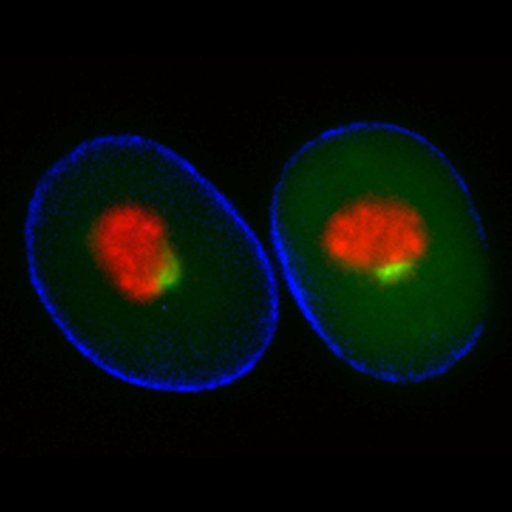
\includegraphics[width=0.80\columnwidth]{./figs/_1colr.jpg}
 \caption{Input image 1. \cite{cil:9233}}
  \label{fig:inputimage1}
\end{subfigure}%
\begin{subfigure}{.48\textwidth}
  \centering
  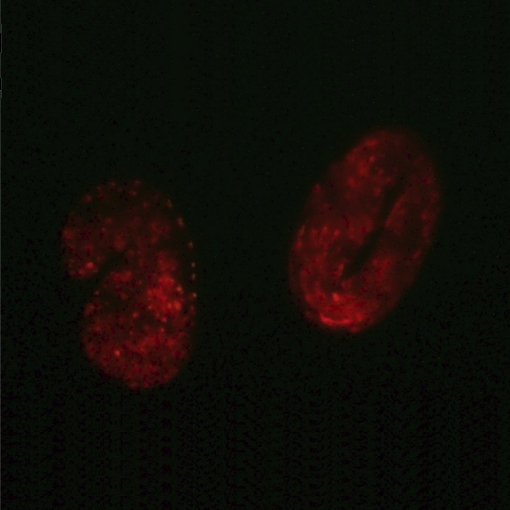
\includegraphics[width=0.80\columnwidth]{./figs/_3colr.jpg}
 \caption{Input image 2. \cite{cil:13902}}
  \label{fig:inputimage2}
\end{subfigure}%


\begin{subfigure}{.48\textwidth}
  \centering
  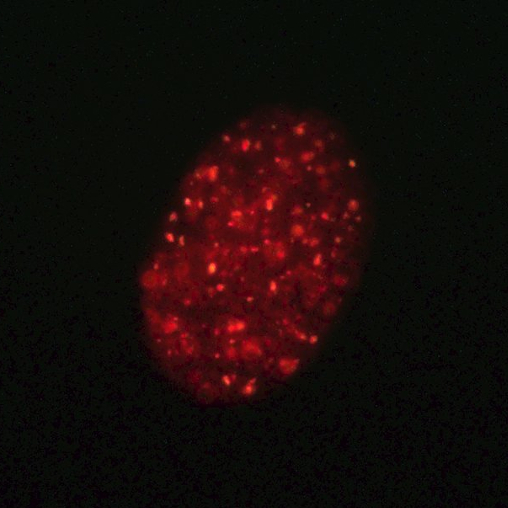
\includegraphics[width=0.80\columnwidth]{./figs/_4colr.jpg}
 \caption{Input image 3. \cite{cil:13903}}
  \label{fig:inputimage3}
\end{subfigure}%
\begin{subfigure}{.48\textwidth}
  \centering
  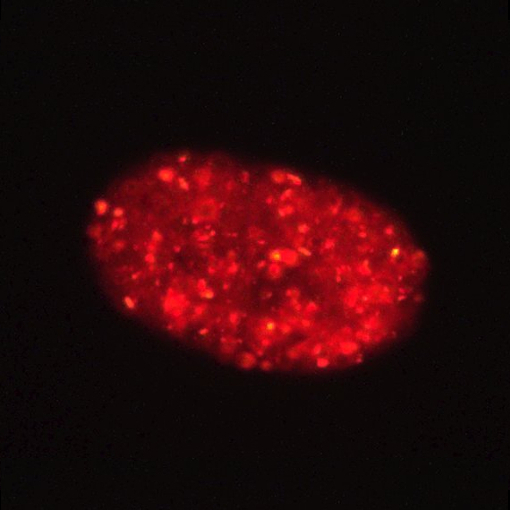
\includegraphics[width=0.80\columnwidth]{./figs/_5colr.jpg}
 \caption{Input image 4. \cite{cil:13904}}
  \label{fig:inputimage4}
\end{subfigure}%
\caption{Input images}
\label{fig:inputimages}
\end{figure}


The output images of the proposed scheme are shown in Figure \ref{fig:outputimages}.
As can be seen, the cells and cell boundaries are more coherent and defined. The segmentations were obtained using the Chan-Vese segmentation via Graph Cuts as presented in \cite{zehiry:2007}. The results of the segmentation are shown in Figure \ref{fig:segmentedimages}. The blue contours denote the ground truth and the red contours are obtained after segmentation.


\begin{figure}[!h]
\centering
\begin{subfigure}{.48\textwidth}
  \centering
  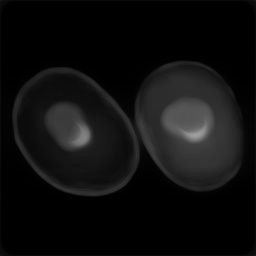
\includegraphics[width=0.80\columnwidth]{./figs/1diffused.jpg}
  \caption{Output Image 1}
  \label{fig:outputimage_1}
\end{subfigure}%
\begin{subfigure}{.48\textwidth}
  \centering
  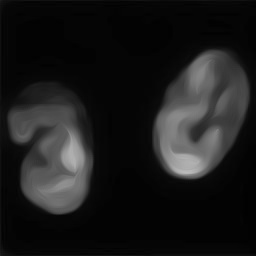
\includegraphics[width=0.80\columnwidth]{./figs/3diffused.jpg}
 \caption{Output Image 2}
  \label{fig:outputimage_3}
\end{subfigure}%


\begin{subfigure}{.48\textwidth}
  \centering
  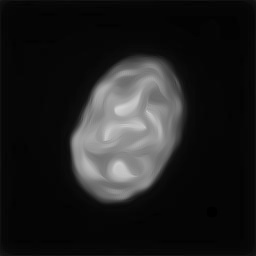
\includegraphics[width=0.80\columnwidth]{./figs/4diffused.jpg}
 \caption{Output Image 3}
  \label{fig:outputimage_4}
\end{subfigure}%
\begin{subfigure}{.48\textwidth}
  \centering
  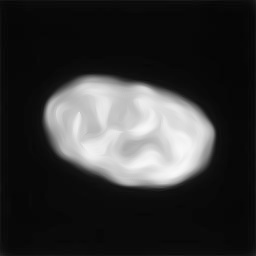
\includegraphics[width=0.80\columnwidth]{./figs/5diffused.jpg}
 \caption{Output Image 4}
  \label{fig:outputimage_5}
\end{subfigure}%
\caption{Output images of proposed scheme}
\label{fig:outputimages}
\end{figure}

\begin{table}
\renewcommand{\arraystretch}{1.3}
\caption{Classification Statistics[A - Original gray scale image, B - CED-ORI only, C - Anisotropic TV denoising only, D - Proposed Preprocessing Scheme]}
\label{tab:class_stats}
\centering
\begin{tabular}{ccccc}
   %& & \multicolumn{3}{c}{} \\ \hline
   \hline
          &   & Sensitivity & Specificity & F1 score\\ \hline
Test Image  	& A & 0.956157 & 0.974129 & 0.975526 \\
 			& B & 0.952542 & 0.971822 & 0.974790 \\
          	& C & 0.778485 & 0.839000 & 0.874881 \\
          	& D & 0.981447 & 0.989360 & 0.987344 \\ \hline

Image 1     	& A & 0.967517 & 0.981730 & 0.979699 \\
	  		& B & 0.972583 & 0.984701 & 0.980968 \\
          	& C & 0.932064 & 0.960116 & 0.963754 \\
          	& D & 0.973092 & 0.985008 & 0.980745 \\ \hline

Image 2     	& A & 0.977581 & 0.997342 & 0.704079 \\
	  		& B & 0.967342 & 0.993423 & 0.945607 \\
          	& C & 0.980888 & 0.996411 & 0.924565 \\
          	& D & 0.973788 & 0.994494 & 0.972452 \\ \hline

Image 3     	& A & 0.984491 & 0.961890 & 0.964425 \\
	  		& B & 0.998658 & 0.999674 & 0.972736 \\
          	& C & 0.878951 & 0.964813 & 0.934818 \\
          	& D & 0.999495 & 0.999873 & 0.989058 \\ \hline

Image 4     	& A & 0.999931 & 0.999980 & 0.966254 \\
	  		& B & 0.997783 & 0.999318 & 0.988121 \\
          	& C & 0.982536 & 0.994460 & 0.988247 \\
          	& D & 1.000000 & 1.000000 & 0.977193 \\ \hline
\end{tabular}
\end{table}

\subsection{Parameter Settings}
The results of the segmentations are presented in \autoref{tab:class_stats}. We compare four pre-processing schemes. In the table, the first scheme is denoted A and represents the results when using the raw gray level image; the  second scheme denoted B represents the results of using the coherence enhancing diffusion filter with optimised rotational invariance (CED-ORI) \cite{jweickert:2002}, as done in \cite{mmaska:2013} and \cite{dkroon:2009}. The parameters used are:
$\sigma = 3.0, \, \rho = 5.0, \, c_1 = 1 \times 10^{-3}, \, c_2 = 1, \, \Delta t = 0.0015, \, n=20$.
The third scheme, denoted  C in the table, is the results of having each image denoised using the following parameters: $\lambda = 1, \, \mu = 20,  \, \epsilon = 1 \times 10^{-3}$.
The fourth scheme, denoted D in the table, is using the proposed scheme. The parameters for the TV denoising and CED-ORI are the same as previously presented. The additional parameters for the third step were set to: $\kappa_1 = 0.17, \, R_1 = 50, \, \kappa_2 = 0.55, \, R_2 = 225$. For the channel mixing step the weights used are shown in \autoref{tab:channel_weights}.

A numerical comparison of each segmentation, in \autoref{tab:class_stats}, shows an increase in the general accuracy of the classification and the segmentation contours are smoother and fit the cell more appropriately.

\begin{table}
\renewcommand{\arraystretch}{1.3}
\caption{Channel Mixing Weights}
\label{tab:channel_weights}
\centering
\begin{tabular}{cccc}
   \hline
           	& $w_R$	& $w_G$	& $w_B$\\ \hline
Test Image  	& 0.2 	& 0.6 	& 0.2 \\ \hline
Image 1     	& 0.5 	& 0.5 	& 0.0 \\ \hline
Image 2		& 1.0 	& 0.0 	& 0.0 \\ \hline
Image 3		& 1.0 	& 0.0 	& 0.0 \\ \hline
Image 4		& 1.0 	& 0.0 	& 0.0 \\ \hline
\end{tabular}
\end{table}

\subsection{Execution Time}
The scheme was implemented in C++ using OpenCV 2.3.4. There were no run-time optimisations performed in the code nor any complexity reduction of algorithms. The Operating System used was Ubuntu 13.10 on a Core 2 Duo 1.3GHz with this 2GB RAM. To get the results, the running times to process 744 images  were analysed. The results are shown in \autoref{tab:results_runningtime}. The mean running time versus the image size can be seen in \autoref{fig:results_runningtime}. As can be seen from \autoref{tab:results_runningtime}, the bulk of the processing time is spent on denoising and intra-region smoothing.


{
{\footnotesize
\begin{table}
\renewcommand{\arraystretch}{1.3}
\caption{Running Time Results}
\label{tab:results_runningtime}
\centering
\begin{tabular}{cccccc}
   %& & \multicolumn{3}{c}{} \\ \hline
   \hline
Chn		& Dims 		& Mean	& St. Dev	& \%TV	& \%CEDORI \\ \hline
1 			& $64\times64$	& $4.63$	& $1.02$	& $24.58$& $74.50$\\
 			& $128\times128$	& $14.44$& $4.02$& $19.12$& $80.61$ \\
          	& $192\times192$	& $31.73$& $8.56$& $22.42$& $77.44$ \\
          	& $256\times256$	& $58.12$& $14.40$& $22.58$& $77.36$ \\
          	& $320\times320$	& $97.72$& $24.91$& $19.86$& $80.09$ \\
          	& $384\times382$	& $147.96$& $37.94$& $18.06$& $81.91$ \\
          	& $448\times448$	& $188.19$& $41.16$& $18.81$& $81.17$ \\
          	& $512\times512$	& $250.24$& $52.16$& $17.68$& $82.30$ \\
          	\hline
          	\multicolumn{4}{r}{Mean} & $20.39$ & $79.42$ \\
          	\multicolumn{4}{r}{St. Dev} & $2.50$ & $2.72$ \\
          	\hline
          	
%          	\hline
2 		 	& $64\times64$	&$5.77$	 &$1.94$	 &$39.45$& $59.78$ \\
 			& $128\times128$	&$17.20$	 &$6.86$ &$32.11$& $67.68$ \\
          	& $192\times6192$&$38.84$	 &$16.02$&$36.63$& $63.27$ \\          			& $256\times256$	&$71.24$	 &$26.47$&$36.84$& $63.11$ \\
          	& $320\times320$ &$117.12$&$42.02$&$33.14$	& $66.83$ \\
          	& $384\times384$ &$174.68$&$60.64$&$30.59$	& $69.83$ \\
          	& $448\times448$ &$223.59$&$69.34$&$31.66$	& $68.32$ \\
          	& $512\times512$ &$294.50$&$86.74$&$30.05$	& $69.93$ \\
          	\hline
          	\multicolumn{4}{r}{Mean} & $33.81$ & $66.04$ \\
          	\multicolumn{4}{r}{St. Dev} & $3.41$ & $3.59$ \\
          	\hline
          	
%            	\hline
3 		  	& $64\times64$ 	&$6.91$ &$2.85$ & $49.42$	&$49.92$ \\
 			& $128\times128$ &$19.96$ &$9.69$ &$41.50$	&$58.32$ \\
          	& $192\times192$ &$45.96$ &$23.49$ &$46.44$&$53.47$ \\
          	& $256\times256$	&$84.37$ &$38.54$ &$46.66$&$53.29$ \\
          	& $320\times320$ &$136.53$&$59.14$ &$42.64$&$57.33$ \\
          	& $384\times382$ &$201.40$&$83.34$ &$39.80$&$60.18$ \\
          	& $448\times448$ &$258.98$&$97.52$ &$41.00$&$58.98$ \\
          	& $512\times512$ &$338.75$&$121.32$&$39.19$&$60.80$ \\
          	\hline
          	\multicolumn{4}{r}{Mean} & $43.33$ & $56.54$ \\
          	\multicolumn{4}{r}{St. Dev} & $3.72$ & $3.87$ \\
          	\hline
\end{tabular}
\end{table}
}

\begin{figure}
\centering
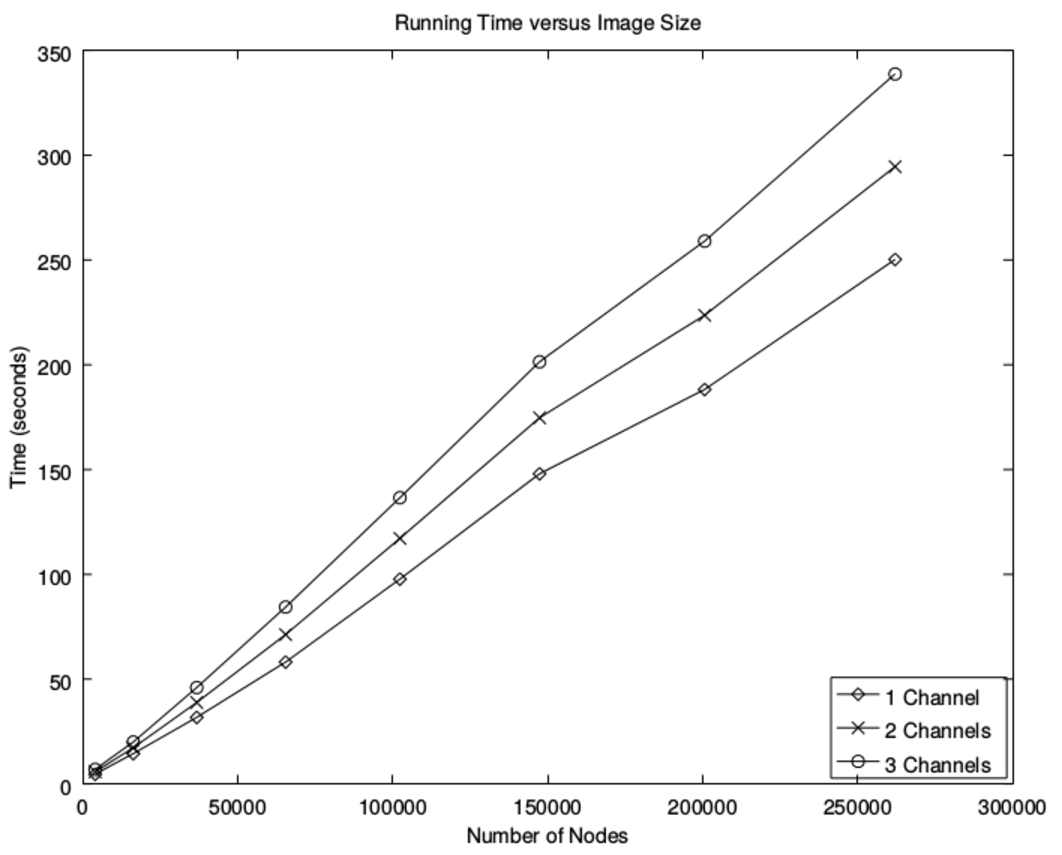
\includegraphics[width=0.80\columnwidth]{./figs/runningtime}
\caption{Running time vs Image size}
\label{fig:results_runningtime}
\end{figure}

\begin{figure*}
\centering
\begin{subfigure}{.25\textwidth}
  \centering
  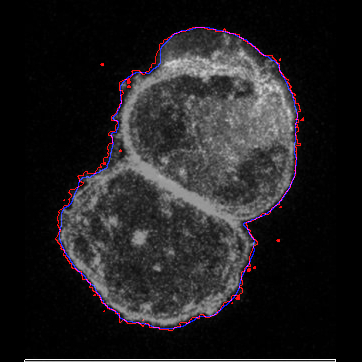
\includegraphics[width=0.80\columnwidth]{./figs/results/2no.jpg}
 \caption{No scheme}
  \label{fig:noseg_2}
\end{subfigure}%
\begin{subfigure}{.25\textwidth}
  \centering
  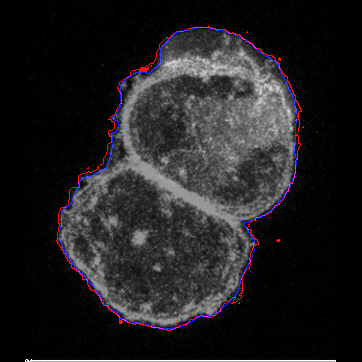
\includegraphics[width=0.80\columnwidth]{./figs/results/2ced.jpg}
 \caption{CED-ORI}
  \label{fig:cedseg_2}
\end{subfigure}%
\begin{subfigure}{.25\textwidth}
  \centering
  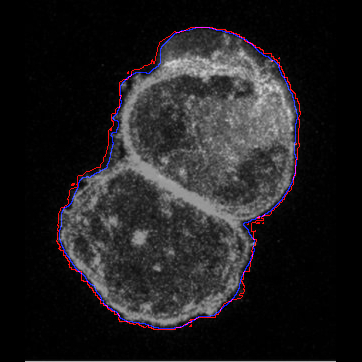
\includegraphics[width=0.80\columnwidth]{./figs/results/2tv.jpg}
 \caption{TV Denoise}
  \label{fig:tvseg_2}
\end{subfigure}%
\begin{subfigure}{.25\textwidth}
  \centering
  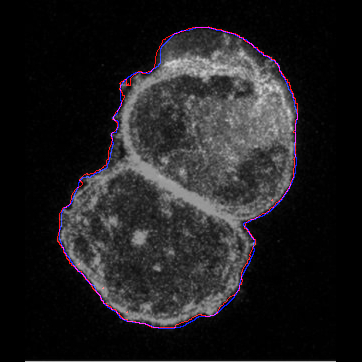
\includegraphics[width=0.80\columnwidth]{./figs/results/2scheme.jpg}
 \caption{Proposed Scheme}
  \label{fig:schemeseg_2}
\end{subfigure}%


\begin{subfigure}{.25\textwidth}
  \centering
  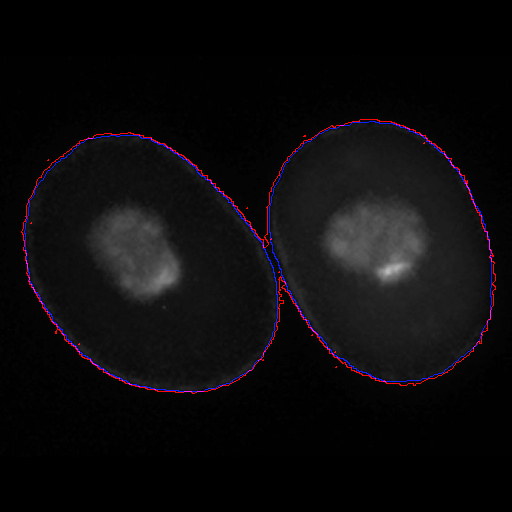
\includegraphics[width=0.80\columnwidth]{./figs/results/1no.jpg}
 \caption{No scheme}
  \label{fig:noseg_1}
\end{subfigure}%
\begin{subfigure}{.25\textwidth}
  \centering
  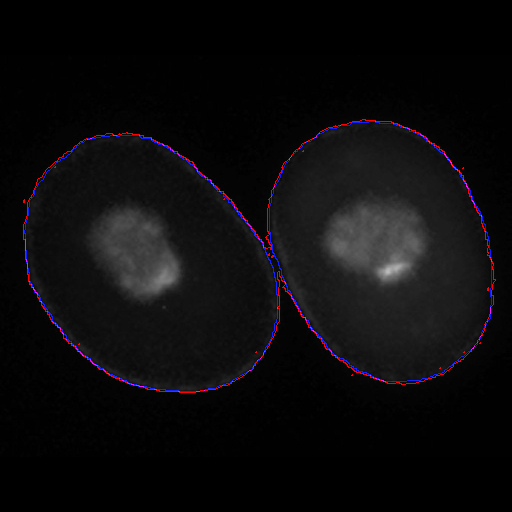
\includegraphics[width=0.80\columnwidth]{./figs/results/1ced.jpg}
 \caption{CED-ORI}
  \label{fig:cedseg_1}
\end{subfigure}%
\begin{subfigure}{.25\textwidth}
  \centering
  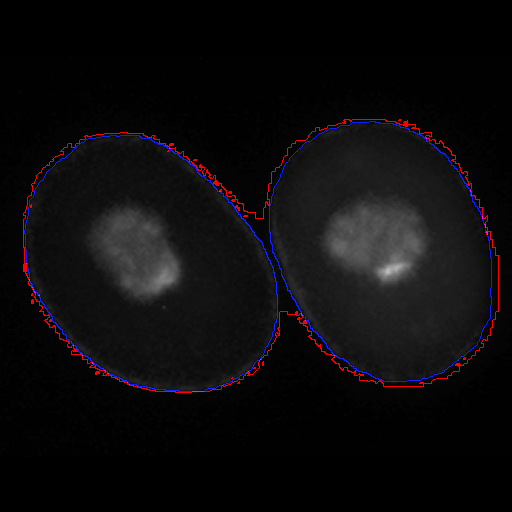
\includegraphics[width=0.80\columnwidth]{./figs/results/1tv.jpg}
 \caption{TV Denoise}
  \label{fig:tvseg_1}
\end{subfigure}%
\begin{subfigure}{.25\textwidth}
  \centering
  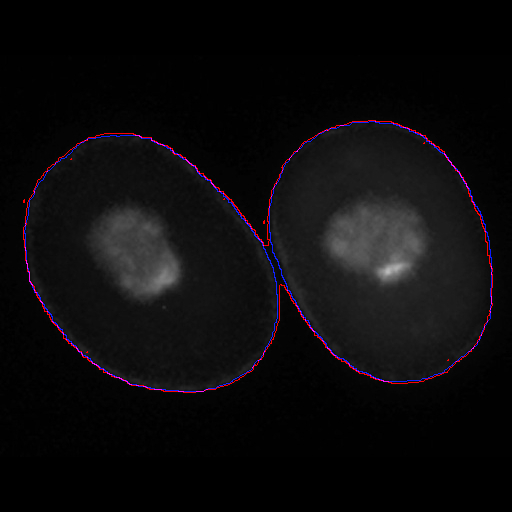
\includegraphics[width=0.80\columnwidth]{./figs/results/1scheme.jpg}
 \caption{Proposed Scheme}
  \label{fig:schemeseg_1}
\end{subfigure}%


\begin{subfigure}{.25\textwidth}
  \centering
  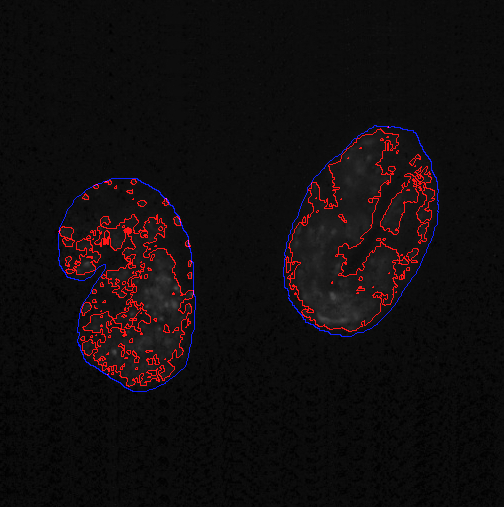
\includegraphics[width=0.80\columnwidth]{./figs/results/3no.jpg}
 \caption{No scheme}
  \label{fig:noseg_3}
\end{subfigure}%
\begin{subfigure}{.25\textwidth}
  \centering
  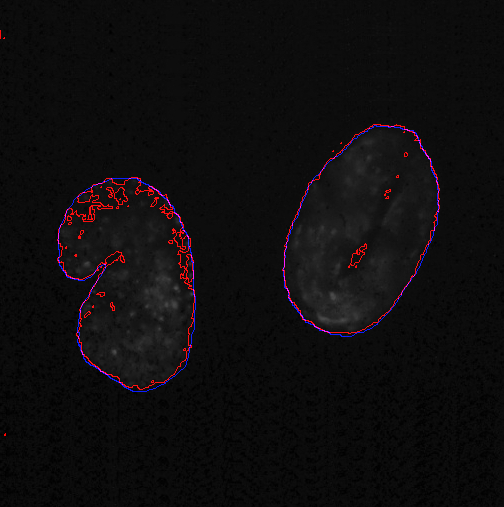
\includegraphics[width=0.80\columnwidth]{./figs/results/3ced.jpg}
 \caption{CED-ORI}
  \label{fig:cedseg_3}
\end{subfigure}%
\begin{subfigure}{.25\textwidth}
  \centering
  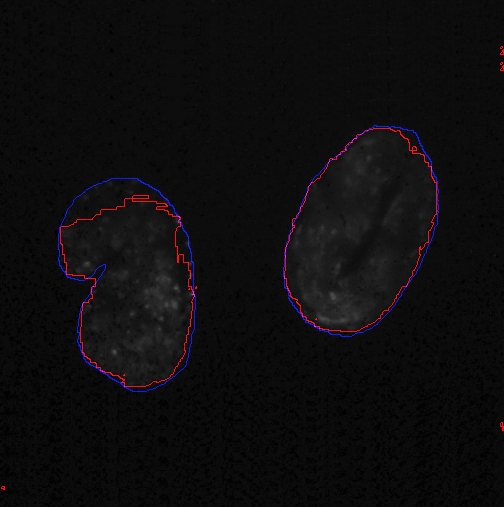
\includegraphics[width=0.80\columnwidth]{./figs/results/3tv.jpg}
 \caption{TV Denoise}
  \label{fig:tvseg_3}
\end{subfigure}%
\begin{subfigure}{.25\textwidth}
  \centering
  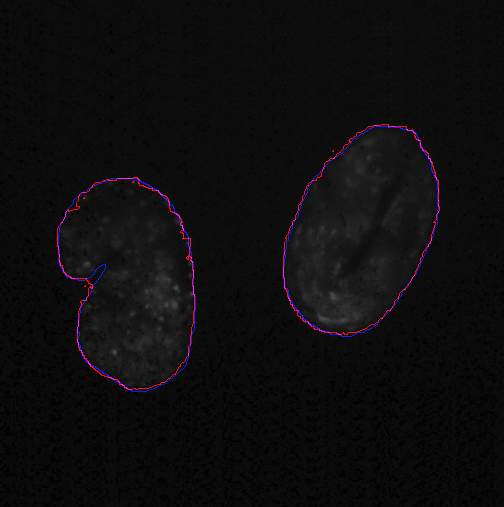
\includegraphics[width=0.80\columnwidth]{./figs/results/3scheme.jpg}
 \caption{Proposed Scheme}
  \label{fig:schemeseg_3}
\end{subfigure}%


\begin{subfigure}{.25\textwidth}
  \centering
  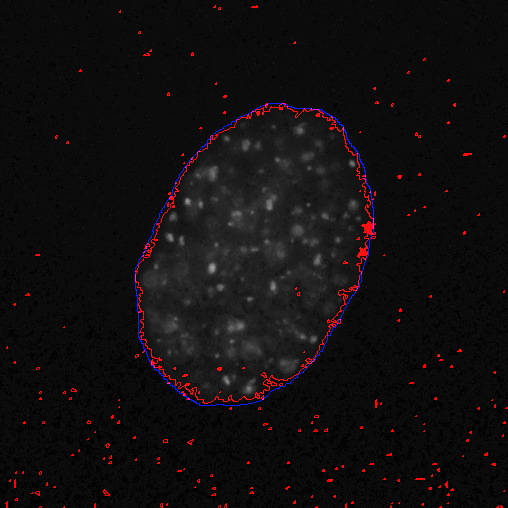
\includegraphics[width=0.80\columnwidth]{./figs/results/4no.jpg}
 \caption{No scheme}
  \label{fig:noseg_4}
\end{subfigure}%
\begin{subfigure}{.25\textwidth}
  \centering
  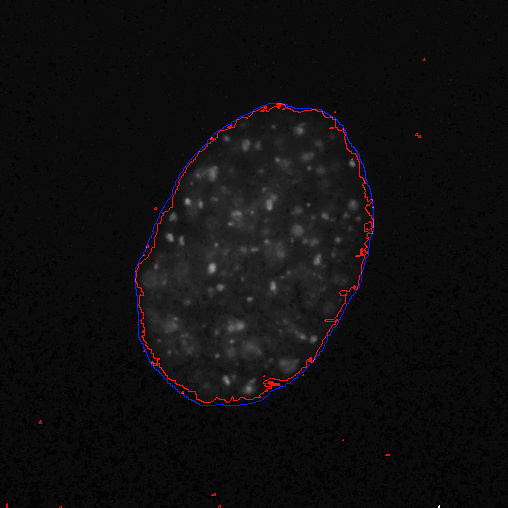
\includegraphics[width=0.80\columnwidth]{./figs/results/4ced.jpg}
 \caption{CED-ORI}
  \label{fig:cedseg_4}
\end{subfigure}%
\begin{subfigure}{.25\textwidth}
  \centering
  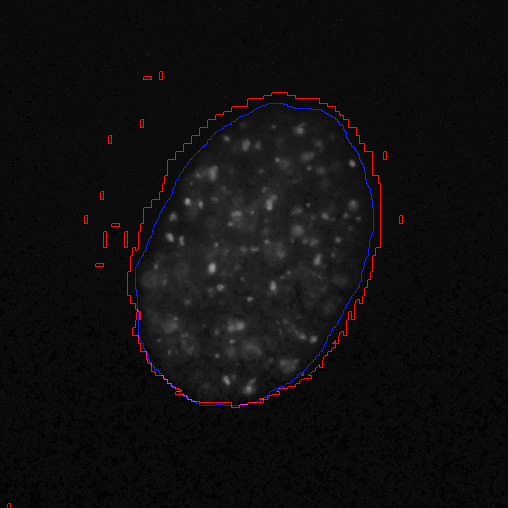
\includegraphics[width=0.80\columnwidth]{./figs/results/4tv.jpg}
 \caption{TV Denoise}
  \label{fig:tvseg_4}
\end{subfigure}%
\begin{subfigure}{.25\textwidth}
  \centering
  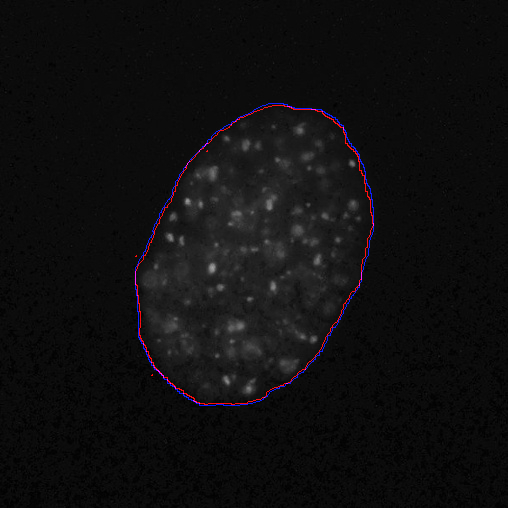
\includegraphics[width=0.80\columnwidth]{./figs/results/4scheme.jpg}
 \caption{Proposed Scheme}
  \label{fig:schemeseg_4}
\end{subfigure}%


\begin{subfigure}{.25\textwidth}
  \centering
  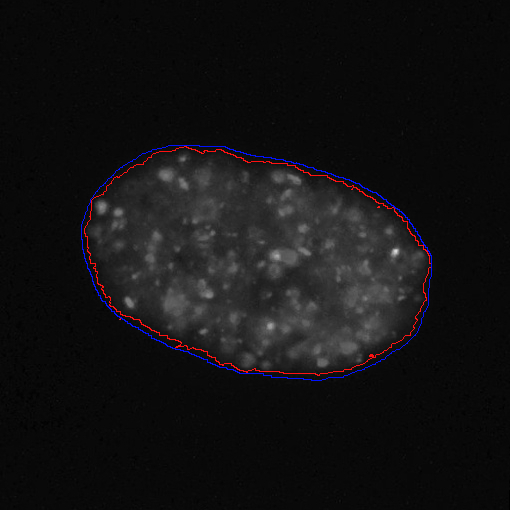
\includegraphics[width=0.80\columnwidth]{./figs/results/5no.jpg}
 \caption{No scheme}
  \label{fig:noseg_5}
\end{subfigure}%
\begin{subfigure}{.25\textwidth}
  \centering
  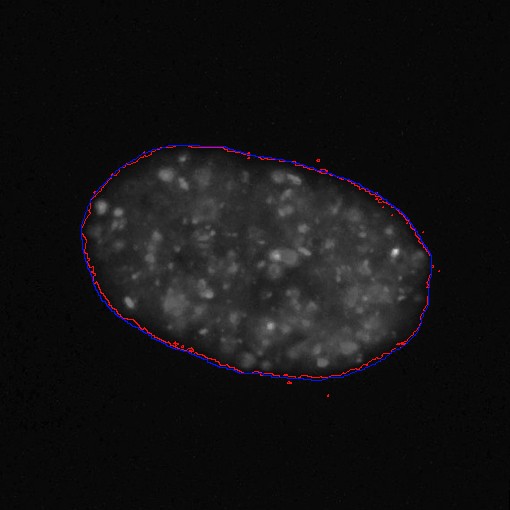
\includegraphics[width=0.80\columnwidth]{./figs/results/5ced.jpg}
 \caption{CED-ORI}
  \label{fig:cedseg_5}
\end{subfigure}%
\begin{subfigure}{.25\textwidth}
  \centering
  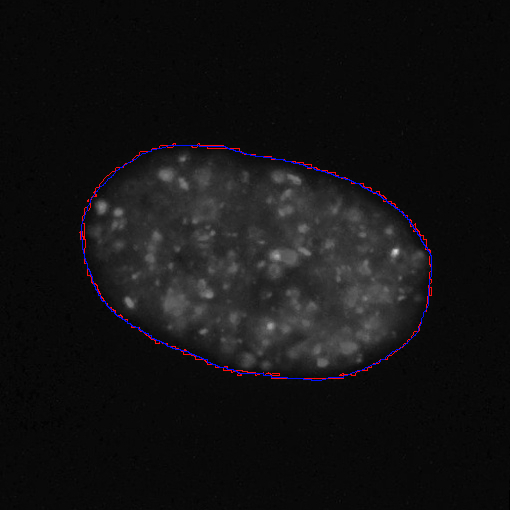
\includegraphics[width=0.80\columnwidth]{./figs/results/5tv.jpg}
 \caption{TV Denoise}
  \label{fig:tvseg_5}
\end{subfigure}%
\begin{subfigure}{.25\textwidth}
  \centering
  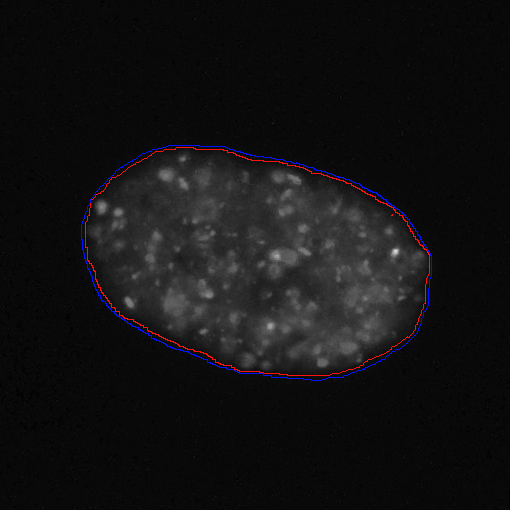
\includegraphics[width=0.80\columnwidth]{./figs/results/5scheme.jpg}
 \caption{Proposed Scheme}
  \label{fig:schemeseg_5}
\end{subfigure}%
\caption{Segmentation Results}
\label{fig:segmentedimages}
\end{figure*}

\section{Conclusion}
\label{sec:conclusion}
We have  presented a scheme that adjusts the properties of an image such that more accurate segmentation can be obtained. Experiments  performed on 2D fluorescence microscopy image data show that the proposed scheme outperforms the existing techniques. One  limitation of the scheme  is the tuning of the various parameters. The running time can also be reduced by  using parallel computing or by optimizing algorithms used.

\bibliographystyle{dcu}
\bibliography{references}

%%%%%%%%%%%%%%%%%%%%%%%%%%%%%%%%%%%%%%%%%%%%%%%%%%%%%%%

\end{document}
